%!TEX root=main.tex
\section{Evaluation}
\label{sec:eval}

\subsection{Testbed and methodology}

We evaluate \name\ in a testbed of 16 Dell R720 servers (\S\ref{subsec:sysarch}).
For each FPGA board, both Ethernet ports are connected to a Top-of-Rack (ToR) Dell S6000 switch~\cite{dells6000}.
All \name\ NFs are running on a Windows Server 2012 R2.
%
We compare \name\ with other state-of-the-art software NFs. 
For those NFs running on Linux, we use CentOS 7.2 with kernel version 3.10.
% delay measurement
In our test, we use PktGen to generate testing traffic at different rates 
with various packet sizes (up to 56.4~Mpps with 64B packets).
%
To measure the NF processing latency, we embed a generation timestamp in every testing packet.
When packets pass the NF, they are looped back to a PktCap which is located with PktGen 
in the same FPGA. 
%
Then we can determine the latency by subtracting the generation timestamp from the receiving 
time of the packet. 
%
The delay induced by the PktGen and PktCap was pre-calibrated via direct loop-back (without NFs) and removed from our data.

\egg{
To measure NF processing latency, we forward packets to an \textit{Echo} server using the second port. 
The Echo server runs an \textit{Echo} function in its FPGA, which simply bounces all packets back to the source. 
%
Then, we can compare the difference between the timestamps of a packet 
when it first arrives and when the processed packet is bounced back, to obtain the latency 
with nanosecond accuracy.
%
The delay induced by the Echo server was pre-calibrated and removed from our data.
In our test, we use PktGen to generate testing traffic, which can 
generate packets at up to 56.4 Mpps (64B packets).
}

\egg{
Ethernet ports of FPGAs and servers are connected to a Dell S6000 40GbE switch 
FPGAs are installed on Windows Server 2012 R2.
CPU-based benchmarks are performed on 

We use TrafficGen application to benchmark throughput and latency.
TrafficGen application generates a given traffic pattern or replays a trace, embeds timestamp in packet payload and sends to tor\_out.
Applications forward packets from tor\_in to nic\_out. When TrafficGen receives packet from nic\_in, the timestamp is extracted from payload to measure latency.
The wire loopback RTT of TrafficGen is 0.85$\mu$s for 64B packets and 1.39$\mu$s for 1504B packets, which is the system error in all latency numbers we present.
}

\begin{figure*}[t!]
	\centering
	\begin{minipage}{.6\textwidth}
		\centering
		\subfigure[]{
			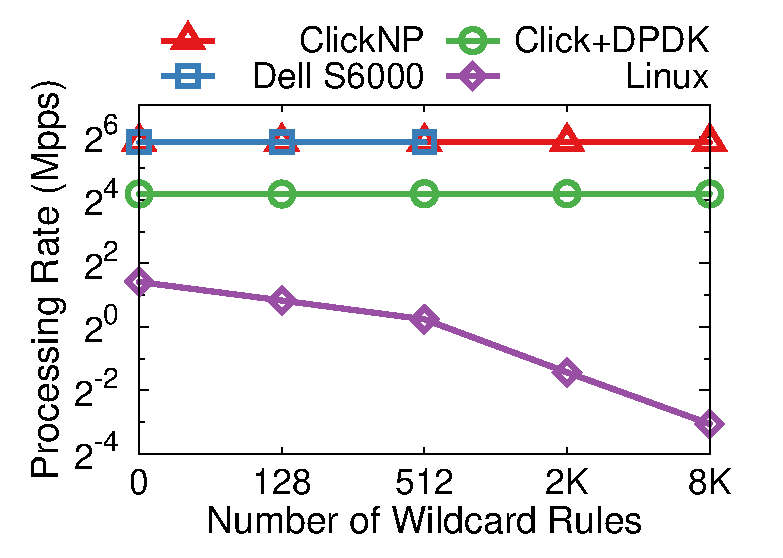
\includegraphics[width=0.45\textwidth]{eval/fw_1}
		}
	%	\subfigure[]{
	%		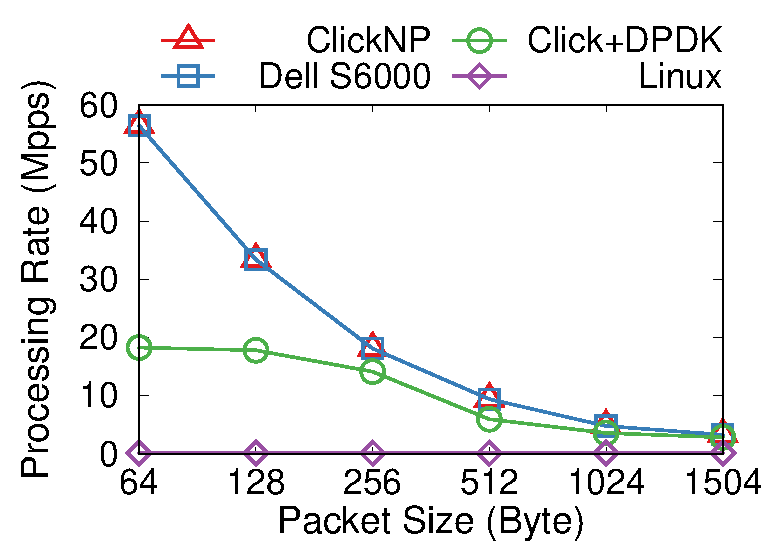
\includegraphics[width=0.225\textwidth]{eval/fw_2}
	%	}
		\subfigure[]{
			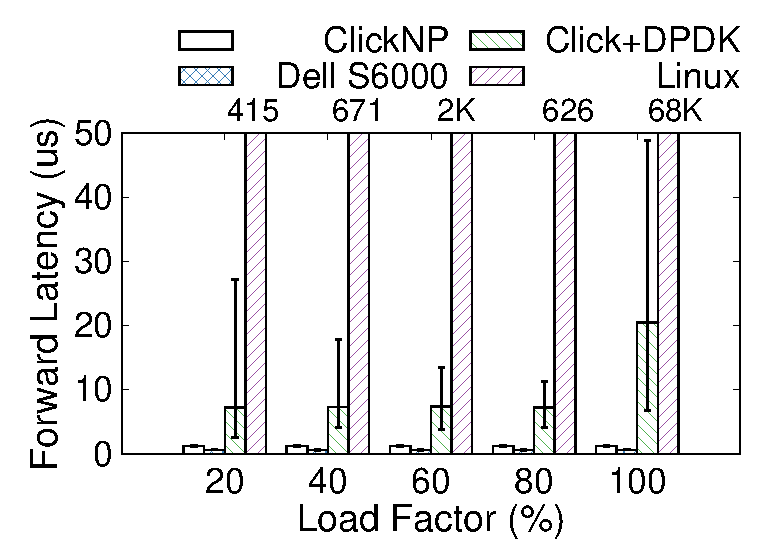
\includegraphics[width=0.45\textwidth]{eval/fw_3}
		}
		\subfigure[]{
			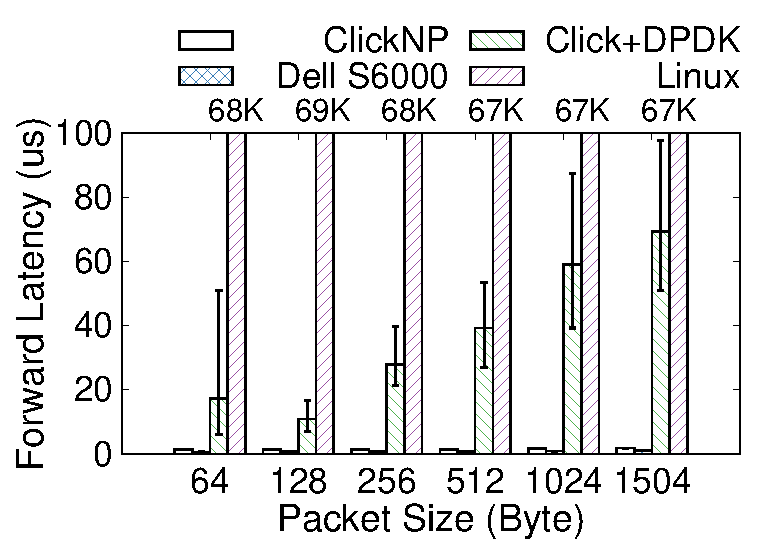
\includegraphics[width=0.45\textwidth]{eval/fw_4}
		}
		\subfigure[]{
			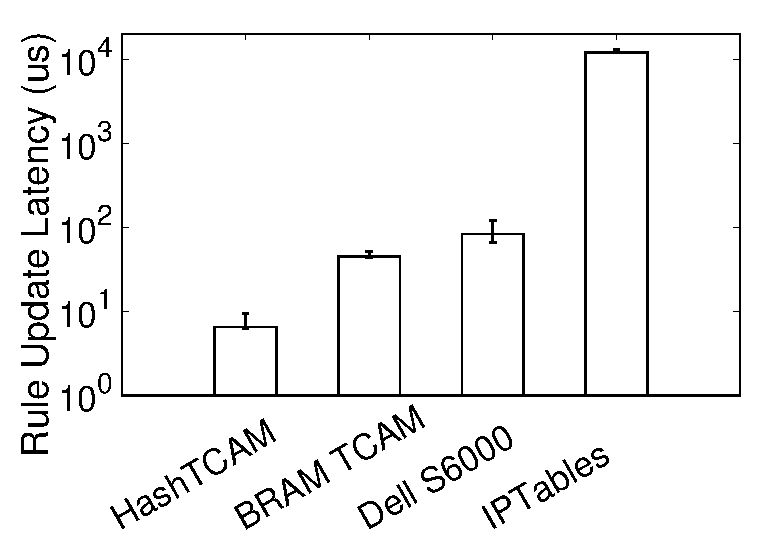
\includegraphics[width=0.45\textwidth]{eval/fw_5}
		}
		\vspace{-10pt}
		\caption{Firewalls. Error bars represents the $5^{th}$ and $95^{th}$ percentile. (a) and (b) Packet size is 64B.}
		\vspace{-10pt}
		\label{fig:firewall}
	\end{minipage}
	\begin{minipage}{.3\textwidth}
		\centering
		\subfigure[]{
			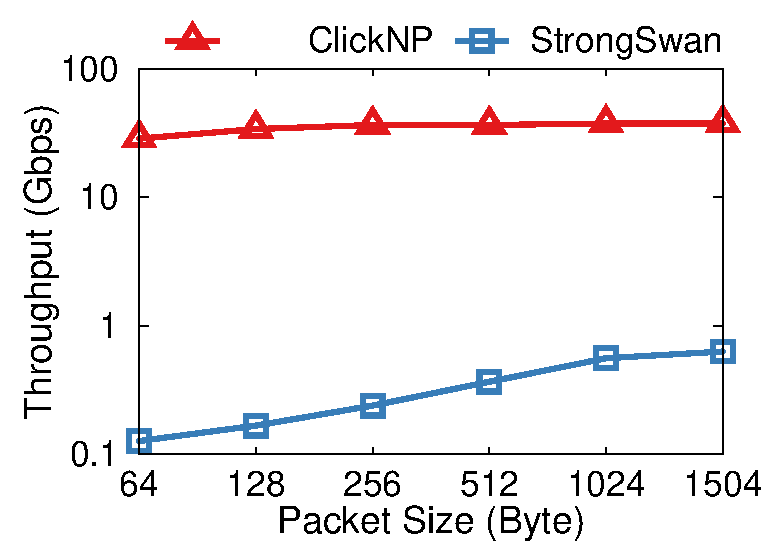
\includegraphics[width=0.9\textwidth]{eval/ipsec_1}
		}
		\subfigure[]{
			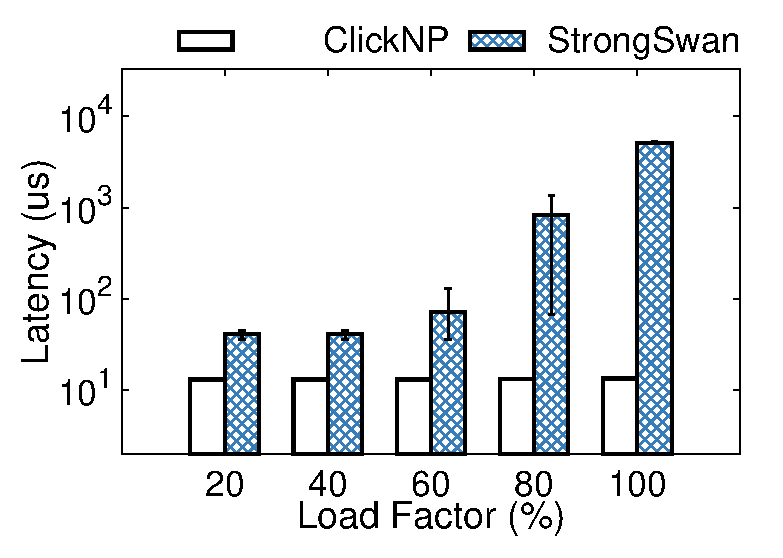
\includegraphics[width=0.9\textwidth]{eval/ipsec_2}
		}
		\vspace{-10pt}
		\caption{IPSec gateway. }
		\vspace{-10pt}
		\label{fig:IPSec}
	\end{minipage}
\end{figure*}

\subsection{Throughput and latency}

%In this subsection, we benchmark the throughput and latency of \name\ NFs.

\smalltitle{OpenFlow firewall.} 
In this experiment, we compare OFW with Linux firewall as well as Click+DPDK~\cite{barbette2015fast}.
For Linux, we use IPSet to handle exact-match rules, while use IPTables for wildcard rules.
As a reference, we also include the performance of Dell S6000 switch, which has limited firewall capability 
and supports 1.7K wild-card rules.
It is worth noting that the original Click+DPDK~\cite{barbette2015fast} does not support Receive Side Scaling(RSS).
In this work, we have fixed this issue and find when using 4 cores, Click+DPDK already achieves the best performance. 
But for Linux, we use as many cores as possible (up to 8 due to RSS limitation) for best performance. 

Figure~\ref{fig:firewall}(a) shows packet processing rates of different firewalls with different number of wild-card rules.
The packet size is 64B.
We can see that both \name\ and S6000 can achieve a maximum speed of 56.4~Mpps. 
Click+DPDK can achieve about 18~Mpps. 
Since Click uses a static classification tree to implement wildcard-match, the processing speed 
does not change with the number of rules inserted. 
%
Linux IPTables has a low processing speed of 2.67~Mpps, and the speed decreases as the number of rules
increases. This is because IPTables performs linear matching for wild-card rules.

Figure~\ref{fig:firewall}(b) shows the processing latency under different loads with small packets (64B) and 8K rules. 
Since each firewall has significantly different capacity, the load factor is normalized to the maximum processing speed of each system. 
%
Under all levels of load, FPGA (\name) and ASIC (S6000) solutions have $\mu$s-scale latency (1.23$\mu$s for ClickNP and 0.62$\mu$s for S6000) with very low variance (1.26$\mu$s for ClickNP and 0.63$\mu$s for S6000 at 95\% percentile).
However, the software solutions have much larger delay, and also much larger variance. 
For example, with Click+DPDK, when the load is high, the latency can be as high as $50\mu s$.
%
Figure~\ref{fig:firewall}(c) shows the processing latency with different packet sizes and 8K rules.
With software solutions, the latency increases with the packet size, mainly due to the larger 
memory to be copied.
In contrast, FPGA and ASIC retain the same latency irrespective to the packet size. 
In all experiments, the CPU usage of \name\ OFW is very low ($<5\%$ of a core).

Finally, Figure~\ref{fig:firewall}(d) shows rule insertion latency when there are already 8K rules. Click's static classification tree requires a prior knowledge of all rules, and generating tree for 8K rules takes one minute.
IPTables rule insertion takes 12ms, which is proportional to the number of existing rules in the table.
Rule insertion in Dell S6000 takes 83.7$\mu$s.
For \name, inserting a rule into HashTCAM table takes 6.3\approx9.5$\mu$s for 2\approx3 PCIe round-trips, while SRAM TCAM table takes 44.9$\mu$s on average to update 13 lookup tables.
\name\ data plane throughput does not degrade during rule insertion.
We conclude that OFW has similar performance as ASIC in packet processing, but is flexible and reconfigurable.



\smalltitle{IPSec gateway.} We compare IPSecGW with StrongSwan~\cite{strongswan}, using the same cipher suite of
AES-256-CTR and SHA1. We setup one IPSec tunnel and Figure~\ref{fig:IPSec}(a) shows the throughput with different packet sizes.
With all sizes, IPSecGW achieves line rates, \ie, 28.8Gbps with 64B packets and 37.8 Gbps with 1500B packets. 
%
StrongSwan, however, achieves only a maximum of 628Mbps, and the throughput decreases as packets become smaller.
This is because with smaller size, the number of packets needed to be processed increases, 
and therefore the system needs to compute more SHA1 signatures.
%
Figure~\ref{fig:IPSec}(b) shows the latency under different load factors. Again, IPSecGW yields constant latency of 13$\mu$s, 
but StrongSwan incurs larger latency with higher variance, up to 5ms!

\begin{figure*}[t!]
	\centering
	
	\subfigure[]{
		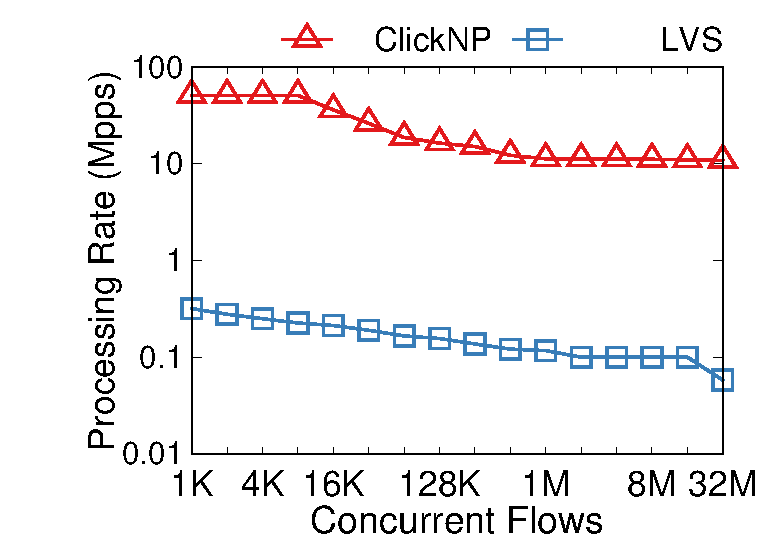
\includegraphics[width=0.3\textwidth,height=0.21\textwidth]{eval/l4_2}
	}
	\subfigure[]{
		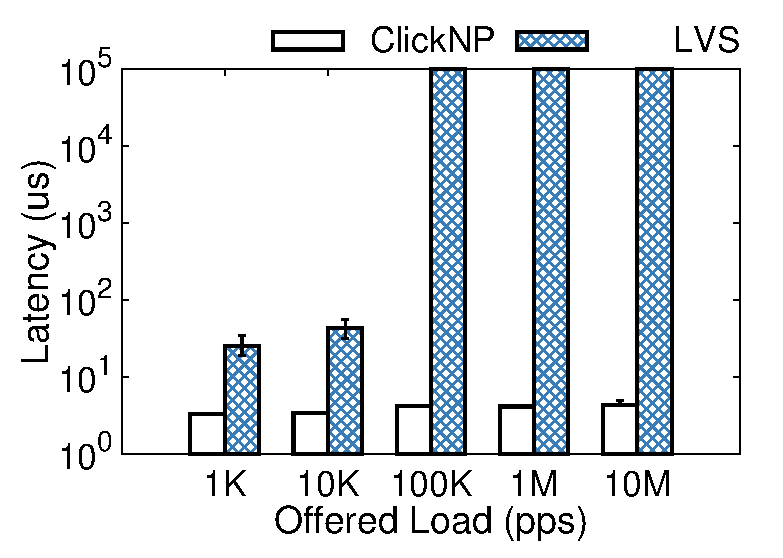
\includegraphics[width=0.3\textwidth]{eval/l4_1}
	}
	\subfigure[]{
		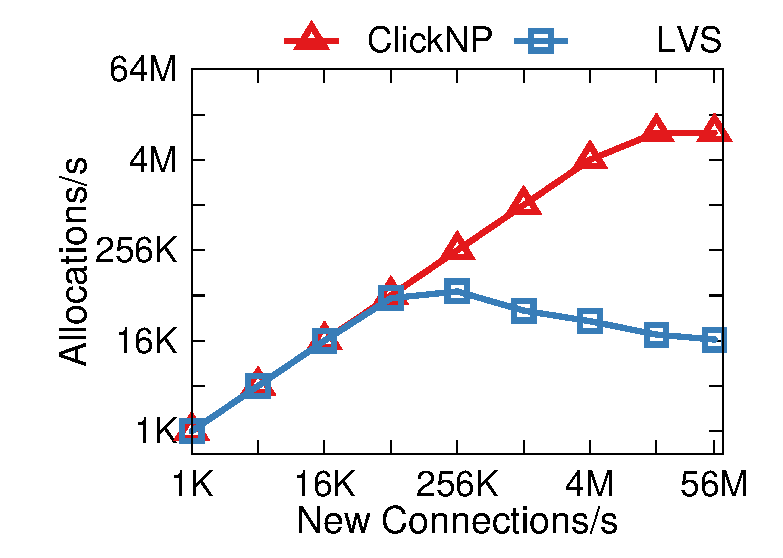
\includegraphics[width=0.3\textwidth]{eval/l4_3}
	}
\vspace{-10pt}
	\caption{L4 Load Balancer.}
	\label{fig:l4}
\vspace{-10pt}
\end{figure*}


\smalltitle{L4 load balancer.} We compare L4LB with Linux Virtual Server (LVS)~\cite{lvs}.
To stress test the system, we generate a large number of concurrent UDP flows with 64B packets, targeting one virtual IP (VIP).
Figure~\ref{fig:l4}(a) shows the processing rates with different number of concurrent flows.
When the number of concurrent flows is less than 8K, L4LB achieves the line rate of 51.2Mpps.
However, when the number of concurrent flows becomes larger, the processing rate starts to drop.
This is because of flow cache misses in L4LB. 
When a flow is missing in the flow cache,  L4LB has to access the onboard DDR memory,
which results in lower performance.
When there are too many flows, \eg, 32M, cache miss dominates and for most of the packets, 
L4LB needs to have one access to the DDR memory. So the processing rate reduces to 11Mpps.
In any case, the processing rate of LVS is low.  
Since LVS associates a VIP to only one CPU core, its processing rate is bound to 200Kpps.

Figure~\ref{fig:l4}(b) shows the latency under different load conditions. 
In this experiment, we fix the number of concurrent flows to 1 million. 
We can see that L4LB achieves very low latency of $4\mu$s.
LVS, however, incurs around $50\mu$s delay.
This delay goes up quickly when the offered load is higher than 100Kpps, which exceeds the  capacity of LVS. 

Finally, Figure~\ref{fig:l4}(c) compares the capability of L4LB and LVS to accept new flows. 
In this experiment, we instruct PktGen to generate as many one-packet tiny flows as possible.
We can see that L4LB can accept up to 10M new flows per second.
%
Since a single PCIe slot can transfer 16.5M flits per second, the bottleneck is still DDR access.
%
Our \textit{DIPAlloc} element simply allocates DIP in a round-robin manner.
For complex allocation algorithms, the CPU core of \textit{DIPAlloc} will be the bottleneck, and the performance can be improved by duplicating \textit{DIPAlloc} elements on more CPU cores.
For LVS, due to the limited packet processing capacity, it can only accept up to 75K new flows per second.

\egg{
\textbf{Stateful L4 load balancer.} We compare our ClickNP implementation with Linux Virtual Server (LVS) \cite{lvs} using both real-world traffic trace on a L4 load balancer \cite{gandhi2014duet} and synthetic traces to simulate adversary scenarios.
The real-world trace contains 1.3M flows collected in two hours with 26Gbps average throughput and 45KB median flow size.
The first adversary trace is round-robin scheduling packets from a large number of infinite UDP flows with 64B packet size to stress the load balancer under high concurrency.
The second adversary trace is a lot of tiny UDP flows to test how many new connections the load balancer can process per second.

Figure \ref{fig:l4} shows that ClickNP L4 load balancer has 50\approx500x lower latency than LVS on real-world trace, supports 32M concurrent flows and able to accept \approx10M new flows per second.
This performance is comparable to high-end hardware load balancers \cite{f5loadbalance}, while ours have low cost and high flexibility.
Figure \ref{fig:l4} also shows the importance of SRAM cache and pipelined DRAM access.
Our board can perform at most 13.6M DRAM random reads per second, and our new flow allocation rate gets near this limit thanks to pipelined DRAM access.
}

\egg{
First we test the performance under real-world data center traffic. We adopted the same traffic trace as DUET\cite{}, and picked the first ten minutes as testing data. Figure \ref{fig:l4} shows the four experiments we performed on the L4 load balancer. We first use TCP traffic to evaluate the flow completion time (FCT) under different throughputs. Then we use UDP traffic to evaluate the latency. 

Next we tested the performance with adversary traffic to thest the worst case performance. We fixed every flow to be one 1504 byte packet, and test the throughput under different flow numbers, and latency under different new flow rates.
}

\subsection{Resource utilization}

In this subsection, we evaluate the resource utilization of \name\ NFs.
Table~\ref{tab:applications} summarizes the results. 
Except for IPSec gateway which uses most BRAMs to hold coding books, 
all other NFs only use moderate resources (5\approx 50\%).  
There is still room to accommodate even more complex NFs.

Next, we study the overhead of fine-grained modularization of \name. 
Since every element will generate a logic block boundary and use only FIFO buffers to communicate with other blocks,
there should be an overhead.
To measure this overhead, we create a simple element that only passes data from one input port to an output port.
The resource utilization of this \textit{empty} element should well capture the overhead of modularization.
Different HLS tools may use different amount of resources, but all are low, with a min of 0.15\% to a max of 0.4\%.
So we conclude \name\ incurs little overhead due to modularization.

Finally, we want to study the efficiency of RTL code generated by \name, compared to hand-written HDL. 
To do so, we use NetFPGA~\cite{netfpga} as our reference.
We extract the key modules in NetFPGA, which are well optimized by experienced Verilog programmers, 
and implement counterpart elements in \name\ with the same functionality. 
We compare the relative area cost between these two implementations using different HLS tools as a backend.
The results are summarized in Table~\ref{tab:netfpga}.
Since different tools may have different area costs, we record both the maximum and minimal value.
%
We can see generally, automatically generated HDL code uses more area compared to hand-optimized code.
The difference, however, is not very large. 
For complex modules (shown in the top part of the table), the relative area cost is less than 2x.
%
For tiny modules (shown in the bottom part of the table), the relative area cost appears larger, but the absolute 
resource usage is small.
This is because all HLS tools
would generate a fixed overhead that dominates the area cost for tiny modules. 

In summary, \name\ can generate efficient RTL for FPGA that incurs only moderate area cost, 
which is capable of building practical NFs.
Looking forward, FPGA technology is still evolving very rapidly. For example, the next
generation FPGA from Altera, Arria 10, would have 2.5x more capacity than the chip we use
currently. 
Therefore, we believe the area cost of HLS would be less of a concern in the future. 

\vspace{10pt}


\egg{
Figure \ref{tab:applications} shows Logic Elements (LE) and BRAM footprint of aforementioned ClickNP applications.
Catapult shell and OpenCL runtime take 30\% LEs and 18\% BRAMs in addition to ClickNP applications.
}

\begin{table}[t!]
	\centering
	\vspace{-5pt}
	\caption{Summary of ClickNP NFs.}
	\label{tab:applications}
	\scalebox{0.9}{
		\begin{tabular}{l|r|r|r|r}
			\toprule
			Network Function & LoC$^\dagger$ & \#Elements & LE & BRAM \\
			\midrule
			\egg{
			Pkt generator & 13 & 6 & 16\% & 12\% \\
			Pkt capture & 12 & 10 & 8\% & 5\% \\
			OpenFlow firewall & 23 & 7 & 32\% & 54\% \\
			IPSec gateway & 37 & 10 & 35\% & 74\% \\
			L4 load balancer & 42 & 13 & 36\% & 38\% \\
			pFabric scheduler & 23 & 7 & 11\% & 15\% \\
			}
			Pkt generator & 665 & 6 & 16\% & 12\% \\
			Pkt capture & 250 & 11 & 8\% & 5\% \\
			OpenFlow firewall & 538 & 7 & 32\% & 54\% \\
			IPSec gateway & 695 & 10 & 35\% & 74\% \\
			L4 load balancer & 860 & 13 & 36\% & 38\% \\
			pFabric scheduler & 584 & 7 & 11\% & 15\% \\
			\bottomrule
			\multicolumn{5}{l}{$^\dagger$ Total line of code of all element declarations and} \\
			\multicolumn{5}{l}{configuration files.}
		\end{tabular}
	}
\vspace{-10pt}
\end{table}

\egg{
To evaluate ClickNP's area cost overhead compared to hand-written HDL, we implemented several ClickNP elements resembling network functions in NetFPGA 10G \cite{netfpga} reference router and Openflow switch projects.
Table \ref{tab:netfpga} compares ClickNP's relative area cost over NetFPGA using Vivado HLS 2015.4 and Altera OpenCL 15.1.
Most ClickNP implementations show less than 100\% logic overhead and less than 30\% BRAM overhead. For tiny elements (\eg IP checksum), a fixed element overhead dominates.
}

\begin{table}[t!]
	\centering
	\vspace{-5pt}
	\caption{Relative area cost compared to NetFPGA.}
	\label{tab:netfpga}
	\scalebox{0.9}{
		\begin{tabular}{l|r|r|r}
			\toprule
			\multirow{2}{2.2cm}{NetFPGA Function} & LUTs & Registers & BRAMs \\
						& Min / Max & Min / Max & Min / Max \\
			\midrule
			Input arbiter  & 2.1x / 3.4x & 1.8x / 2.8x & 0.9x / 1.3x \\
			Output queue   & 1.4x / 2.0x & 2.0x / 3.2x & 0.9x / 1.2x \\
			Header parser  & 0.9x / 3.2x & 2.1x / 3.2x & N/A \\
			Openflow table & 0.9x / 1.6x & 1.6x / 2.3x & 1.1x / 1.2x \\
			\midrule
			\midrule
			IP checksum    & 4.3x / 12.1x & 9.7x / 32.5x & N/A \\
			Encap          & 0.9x / 5.2x & 1.1x / 10.3x & N/A \\
			\bottomrule
		\end{tabular}
	}
\vspace{-10pt}
\end{table}

\egg{
Original data:
Function	LUTs			Registers			BRAMs		
NetFPGA	AOCL	VHLS	NetFPGA	AOCL	VHLS	NetFPGA	AOCL	VHLS
Input arbiter	2048	4346	6998	4553	12843	8348	30	40	26
Output queue	3824	5280	7542	6479	13409	21005	22.5	26	20
Header parser	626	2012	567	698	6095	817	N/A		
Openflow table	3923	6322	3535	4438	10171	7140	33.5	40	38
IP checksum	207	2511	884	162	5269	1576	N/A		
Encap	684	3536	636	821	8493	871	N/A	
}

\subsection{Validation of pFabric}
Before we end this section, we show that \name\ is also a good tool for network research.
Thanks to the flexibility and high performance, we can quickly prototype the latest research 
and apply it to real environments.
For example, we can easily implement pFabric scheduler~\cite{pfabric} using \name, and 
apply it in our testbed.
%
In this experiment, we modify a software TCP flow generator~\cite{mqecn} to place the flow
priority, \ie, the total size of the flow, in packet payload.
We generate flows according to the data-mining workload in~\cite{pfabric} and further
the restrict egress port to be 10~Gbps using a \textit{RateLimit} element.
We apply pFabric to schedule flows in egress buffer according to flow priorities. 
Figure~\ref{fig:pfabric} shows the average flow completion time (FCT) of pFabric, TCP with Droptail queue, and the ideal.
This experiment validates that pFabric achieves near ideal FCT in this simple scenario.

\begin{figure}[h!]
\centering
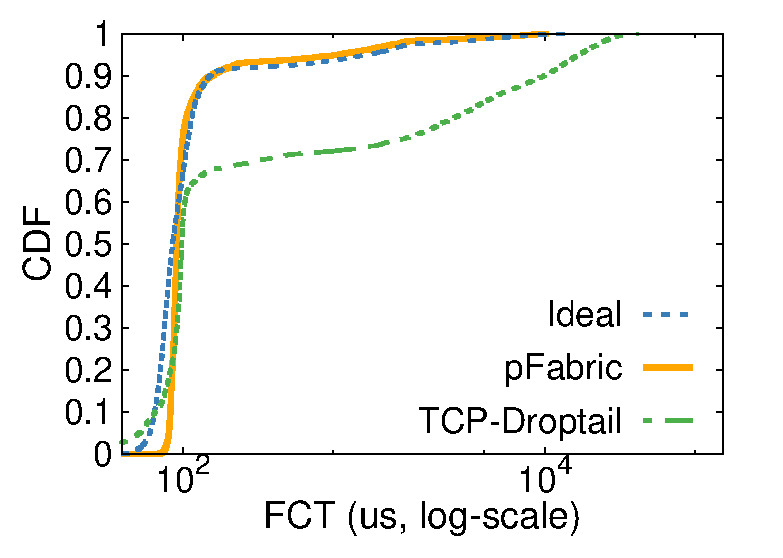
\includegraphics[width=0.3\textwidth]{eval/pfabric}
\vspace{-10pt}
\caption{Validation of pFabric.}
\label{fig:pfabric}
\vspace{-10pt}
\end{figure}


\egg{
\subsection{Network Benchmark Suite}

\subsubsection{Configurable Flow Generator}

\begin{lstlisting}
Rand(0,1,2) -> MetaGen(1,1) -> RevParser(1,1) -> IPChecksum(1,1) -> TCPChecksum(1,1) -> NVGRE_Encap(1,1) -> tor_out
\end{lstlisting}

\subsubsection{Packet Trace Replay}

\begin{figure}[h!]
	\centering
	
\includegraphics[width=0.6\columnwidth]{image/logo}
	\vspace{-0.15in}
	\caption{Traffic Replay Throughput, x: packet size, y: Gbps, lines: ClickNP, CPU}
	\vspace{-0.15in}
	\label{fig:TrafficReplayPerformance}
	%    \vspace{-2mm}
\end{figure}

\subsubsection{Traffic Monitor}

\begin{lstlisting}
tor_in -> Receiver -> Drop (1,0)
\end{lstlisting}

latency, throughput, sequence number check

\subsection{Network Virtualization}

\subsubsection{NVGRE Tunneling}

\begin{figure}[h!]
	\centering
	
\includegraphics[width=0.6\columnwidth]{image/logo}
	\vspace{-0.15in}
	\caption{Tunnel Encap + Decap Performance, x: packet size, y: Gbps, lines: ClickNP, Hyper-V}
	\vspace{-0.15in}
	\label{fig:NVGREPerformance}
	%    \vspace{-2mm}
\end{figure}

\subsubsection{Per-VM Metering and Rate Limiting}

\subsection{Security}

\subsubsection{Network-layer Firewall}

\begin{lstlisting}
Parser :: parser(1,2)
DropPolicer :: action(2,2)
tor_in -> parser[1] -> [1]action[1] -> nic_out
parser[2] -> ExtractFiveTuple(1,1) -> Hashtable @(1,1) -> [2]action[2] -> Drop (1,0)
\end{lstlisting}

\begin{figure}[h!]
	\centering
	
\includegraphics[width=0.6\columnwidth]{image/logo}
	\vspace{-0.15in}
	\caption{Network-layer Firewall Performance, x: \#rules, y: pps, lines: ClickNP, Linux iptables}
	\vspace{-0.15in}
	\label{fig:FirewallPerformance}
	%    \vspace{-2mm}
\end{figure}

\subsubsection{Application-layer Firewall}

\begin{lstlisting}
Parser :: parser(1,2)
DropPolicer :: action(2,2)
tor_in -> parser[1] -> [1]action[1] -> nic_out
parser[2] -> ExtractFiveTuple(1,1) -> RegexMatch @(1,1) -> [2]action[2] -> Drop (1,0)
\end{lstlisting}

\begin{figure}[h!]
	\centering
	
\includegraphics[width=0.6\columnwidth]{image/logo}
	\vspace{-0.15in}
	\caption{Application-layer Firewall Performance, x: \#rules, y: Gbps, lines: ClickNP, snort \cite{roesch1999snort}}
	\vspace{-0.15in}
	\label{fig:WAF_Performance}
	%    \vspace{-2mm}
\end{figure}

\subsubsection{DDoS Detection with Bitmap Sketch}

\begin{lstlisting}
Parser :: parser(1,2)
tor_in -> parser[1] -> nic_out
parser[2] -> ExtractVMID(1,1) -> HashTable @(1,1) -> ExtractSrcIP(1,1) -> BitmapSketch @(1,1) -> Drop (1,0)
\end{lstlisting}

OpenSketch \cite{yu2013software}

\begin{figure}[h!]
	\centering
	
\includegraphics[width=0.6\columnwidth]{image/logo}
	\vspace{-0.15in}
	\caption{Sketch Accuracy, x: \#real flows, y: relative error (\%) with error bar}
	\vspace{-0.15in}
	\label{fig:SketchAccuracy}
	%    \vspace{-2mm}
\end{figure}


\subsection{Scheduling}

\subsubsection{PIAS Tagging}

PIAS \cite{bai2014pias}

\subsubsection{Generic Priority Queue}

pFabric \cite{alizadeh2013pfabric}

\subsubsection{Packet Pacing}

Silo \cite{jang2015silo}

\begin{figure}[h!]
	\centering
	
\includegraphics[width=0.6\columnwidth]{image/logo}
	\vspace{-0.15in}
	\caption{CDF of pacing inaccuracy due to buffer overflow, x: percentile, y: time shift, lines: buffer sizes}
	\vspace{-0.15in}
	\label{fig:PacingAccuracy}
	%    \vspace{-2mm}
\end{figure}

\subsubsection{Timestamping}

TIMELY \cite{mittal2015timely} measures RTT as the signal for congestion control. It requires both receive and send timestamping feature and hardware-generated ACK of recent NICs. Furthermore, since ACKs have already been sent by NIC hardware, OS networking stack needs modifications to avoid generating duplicate ACKs.

With ClickNP we can do the same latency measurement without using a NIC with timestamping feature, and does not require modification to the OS networking stack, as long as the FPGAs at sender and receiver have same clock frequency. The idea is to subtract the latency spent in receiver-side OS networking stack. Upon reception of a data packet, we subtract the timestamp and expects the OS to echo back the timestamp in the ACK packet. When the ACK packet is sent, we add the timestamp, as if we had shifted the initial timestamp by OS processing latency. Pseudo code:

\begin{lstlisting}
.element SendTimestamp {
    .state { uint timestamp = 0; }
    .handler {
        if (input_ready) {
            if (!is_ack_packet())
                set_tsval (timestamp);
            else
                set_tsecr (get_tsecr() + timestamp);
        }
        timestamp ++;
    }
}
.element RecvTimestamp {
    .state { uint timestamp = 0; }
    .handler {
        if (input_ready) {
            if (!is_ack_packet())
                set_tsval (get_tsval() - timestamp);
            else
                set_tsval (timestamp);
        }
    }
}
nic_in -> Parser (1,2) -> SendTimestamp (2,1) -> tor_out
tor_in -> Parser (1,2) -> RecvTimestamp (2,1) -> nic_out
\end{lstlisting}

\begin{figure}[h!]
	\centering
	
\includegraphics[width=0.6\columnwidth]{image/logo}
	\vspace{-0.15in}
	\caption{CDF of measured RTT, x: percentile, y: RTT, lines: hardware ACK (ideal), remove OS latency (close to ideal), not remove OS latency (poor)}
	\vspace{-0.15in}
	\label{fig:TimestampAccuracy}
	%    \vspace{-2mm}
\end{figure}
}

\egg{
Figure~\ref{fig:trafficgen} shows the throughput of \name\ traffic generator and capture. We can see that the generator can
generate packets at line-rate of 40 Gbps. 
When packet size is small ($<256B$), the measured throughput is slightly less than 40 Gbps. We confirm this is due to a
bug in Ethernet MAC in the shell, which may drop a few flits when packet rate is high. 
Figure~\ref{fig:trafficgen}(b) shows the capture performance in packet per second.  

\begin{figure}[t!]
	\centering
	\subfigure[] {
	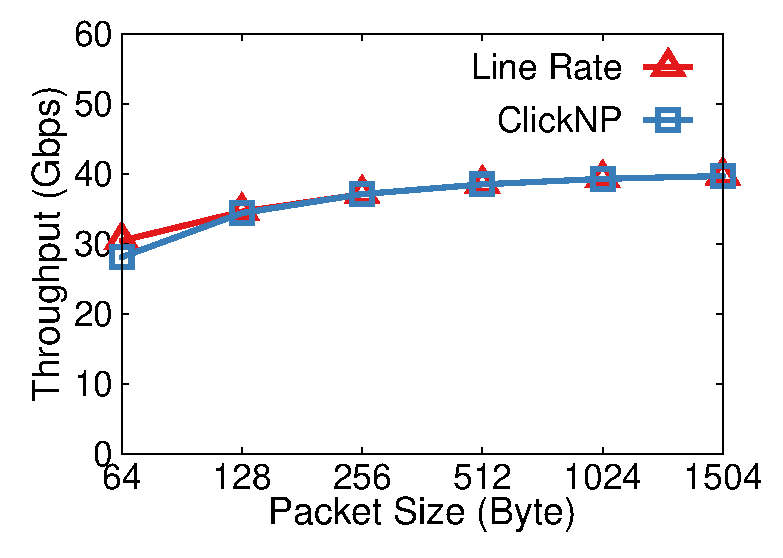
\includegraphics[width=0.225\textwidth]{eval/trafficgen}
	}
	\subfigure[] {
	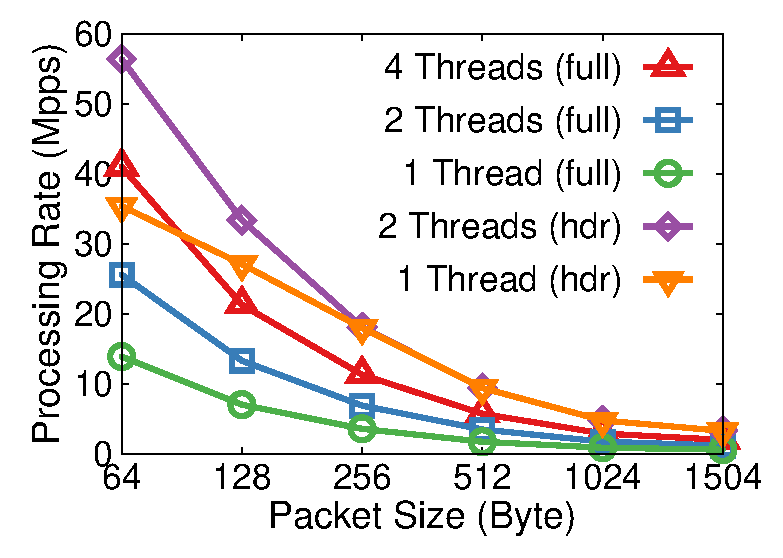
\includegraphics[width=0.225\textwidth]{eval/dump}
	}
	\vspace{-15pt}
	\caption{(a) Traffic generator. (b) Traffic capture.}
	\label{fig:trafficgen}
\end{figure}
}
\egg{
In this section we evaluate throughput and latency of applications presented in section \ref{sec:application}. All these application can achieve line-rate throughput and microsecond-scale latency for reasonable traffic patterns. Latency is averaged over $1000$ rounds, and error bars mark the $5\%$ and $95\%$ percentile.

\textbf{Traffic generator.} We use our traffic generator to send packets to NIC, and use Windows Performance Monitor to measure the throughput. As shown in Figure \ref{fig:trafficgen}, our generator is able to generate packets at 40Gbps line rate when the packet size is not less than 256 bytes. The small gap for 64-byte packets is due to lack of back-pressure in 40GbE MAC of FPGA shell.

\textbf{Traffic capture.} We evaluate the throughput of dumper and results are presented in \ref{fig:dump}.
Each host kernel runs on a separate core and traffic is split evenly to kernels by flow tuple hash.
With four host elements receiving the packets, we can approximately achieve the maximum speed of the PCIe channel.
When we only need the flow tuple and timestamp, ClickNP can easily capture line rate with two cores.
}

\egg{
\textbf{IPSec gateway.} We use StrongSwan \cite{strongswan} with AES256CTR + SHA1 IKEv2 cipher suite as baseline.
After setting up IPSec keys and nonces in ClickNP elements via signal, we send UDP packets in a single IPSec tunnel to test throughput and latency on encryption path.
StrongSwan leverages only one CPU core due to tunnel message sequencing.
As shown in Figure \ref{fig:IPSec}, \textit{Reservo} to exploit packet-level parallelism for SHA-1 element shows 40x performance gain compared to unoptimized version. }

\egg{
\textbf{OpenFlow firewall.} We compare our firewall with Click + DPDK \cite{barbette2015fast} on 4 cores, and Linux iptables (for wildcard match) / ipset \cite{ipset} (for exact match) with RSS on 8 cores.
We also include Dell S6000, a high-end commodity switch, as a reference.

We optimized FromDPDKDevice element in Click to enable receiving packets on multiple cores, while the bottleneck becomes Mellanox polling-mode driver at 18 Mpps.
Click uses a radix tree for exact IP lookup and a classification tree for wildcard flow tuple lookup, so table lookup is not bottleneck of Click.
Linux ipset uses hash table for exact lookup. Linux iptables match wildcard rules linearly, which is the source of low throughput and high latency.
Dell S6000 supports 1.7K 5-tuple wildcard match rules.
For all packet sizes and number of rules, ClickNP offers line rate throughput and latency comparable to commodity ASIC.

Additionally, for 8K wildcard rules, Click takes minutes to generate the classification tree and cannot offer live rule update. ClickNP can perform 350K live rule updates per second while the data plane keeps line forwarding rate. Dell S6000 can perform 12K live rule updates per second.

16K exact, 8 K wild.
}

\egg{
All results are presented in Figure \ref{fig:firewall}. The first two subfigures are to show how packet size and rule numbers influence throughput. In the first subfigure, the packet size is fixed at 64 byte. And in the second subfigure, the numbers of rules is set to be 64k(exact)/8k(wild).

The last two subfigures are about latency. In \ref{}, we fixed the packet size to be ?? and evaluated the latency with different loads. In \ref{}, we change the packet size to see how the latency changes in maximum load scenario. 

From all these figures we can see that ClickNP approximates the performance of Dell S6000, and has a ???x boost on the CPU solution.
}
